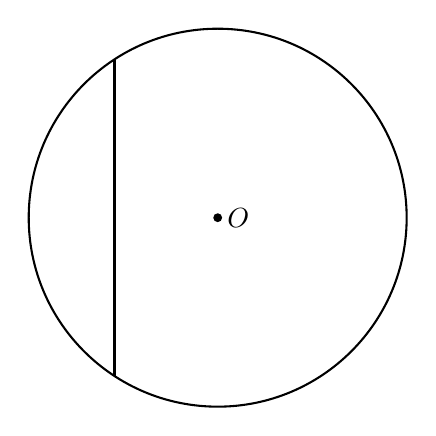
\begin{tikzpicture}[scale=0.8] % Adjust the scale as needed
    % Circle parameters
    \def\r{3} % radius of the circle
    \def\q{5.5} % distance from the center to the external point
    \def\angle{-180} % Rotation angle for the setup

    % x and y coordinates for the tangent points, rotated
    \pgfmathsetmacro{\x}{\r^2/\q} % x coordinate of the point of tangency
    \pgfmathsetmacro{\y}{\r*sqrt(\q^2-\r^2)/\q} % y coordinate of the point of tangency

    % Define points
    \coordinate (O) at (0,0); % Center of the circle
    \coordinate (T1) at ({\x*cos(\angle) - \y*sin(\angle)}, {\x*sin(\angle) + \y*cos(\angle)}); % Tangent point 1, rotated
    \coordinate (T2) at ({\x*cos(\angle) + \y*sin(\angle)}, {\x*sin(\angle) - \y*cos(\angle)}); % Tangent point 2, rotated

    % Draw the circle with radius 3
    \draw[line width=.75pt] (0,0) circle (\r);



    % Draw the diameter
    \draw[line width=1.25pt] (T1) -- (T2);

    % Define a point on the circle for the secant
    \coordinate (Q) at ({-3},{sqrt(\r^2 - 9)}); % Adjust the x-coordinate as needed
        
    % Mark the center of the circle with a dot
    \fill (O) circle (2pt);
    \node at (O) [right] {$O$};
\end{tikzpicture}